\appendix

\begin{frame}{\Large Backup: ViT Gradient Probe}
  \centering
  \vspace{0.12cm}
  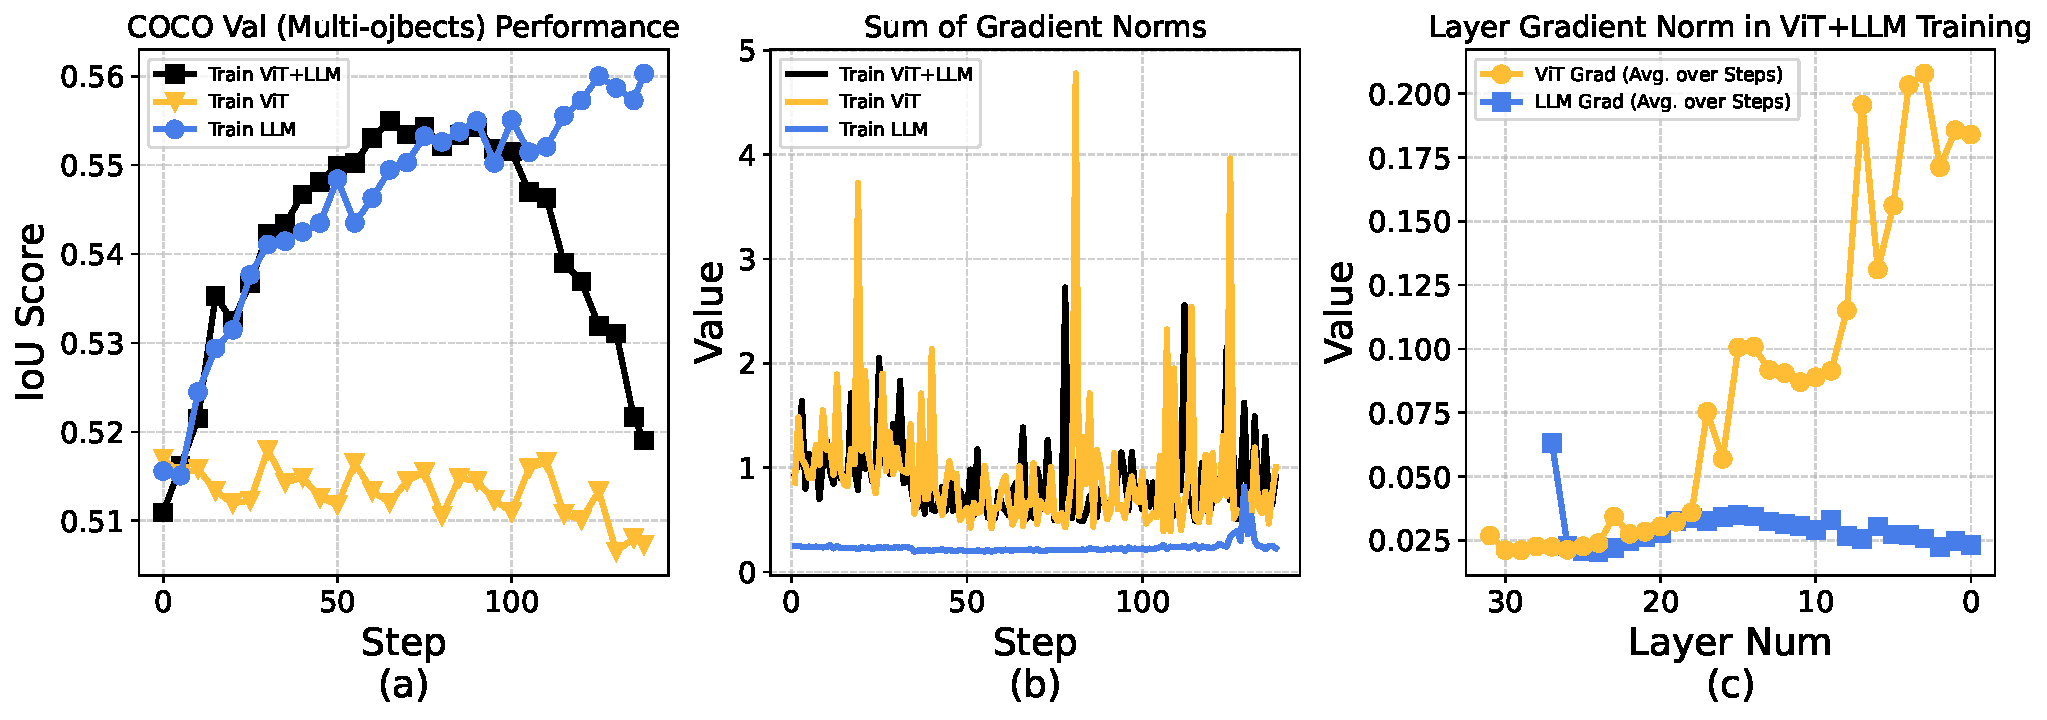
\includegraphics[width=0.80\linewidth]{figures/paper2/disable_vit_full.pdf}
\end{frame}

\begin{frame}{\Large Backup: Ablation Term Curves}
  \centering
  \vspace{0.12cm}
  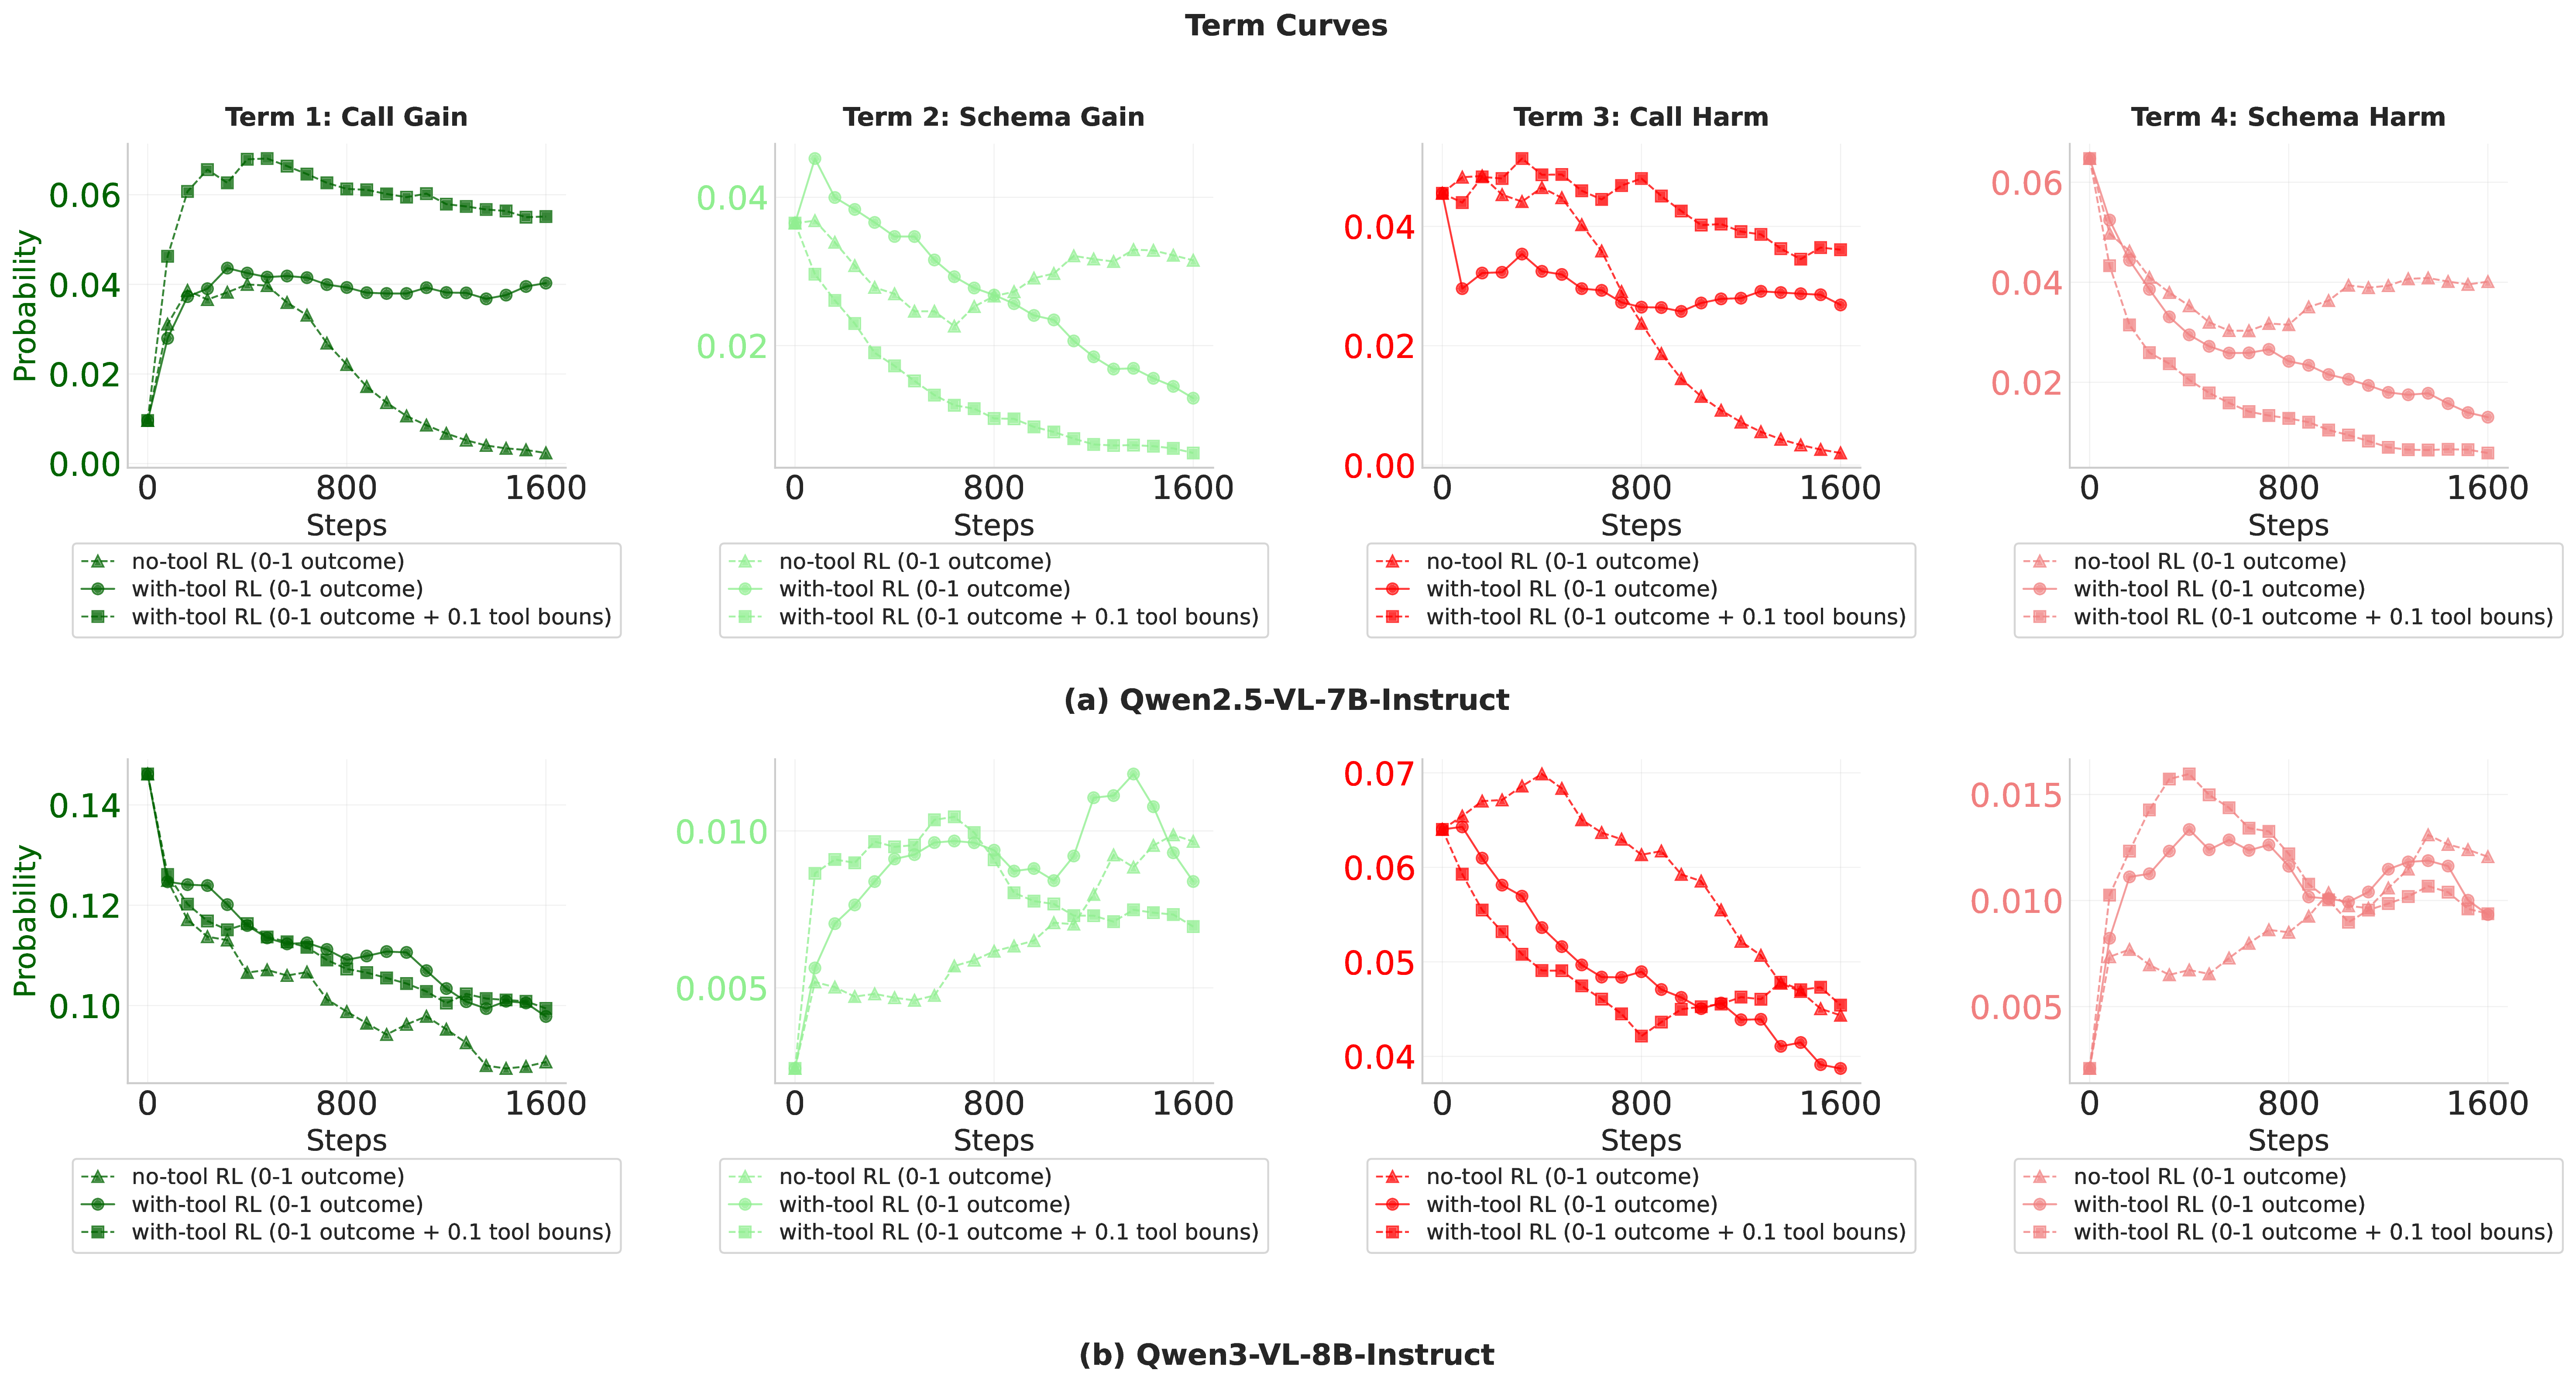
\includegraphics[width=0.98\linewidth]{figures/paper3/baseline_ablation_qwen25vl_qwen3vl_diagnose_term_comparison_terms.png}
\end{frame}

\begin{frame}{\Large Backup: Ablation Factor Curves}
  \centering
  \vspace{0.12cm}
  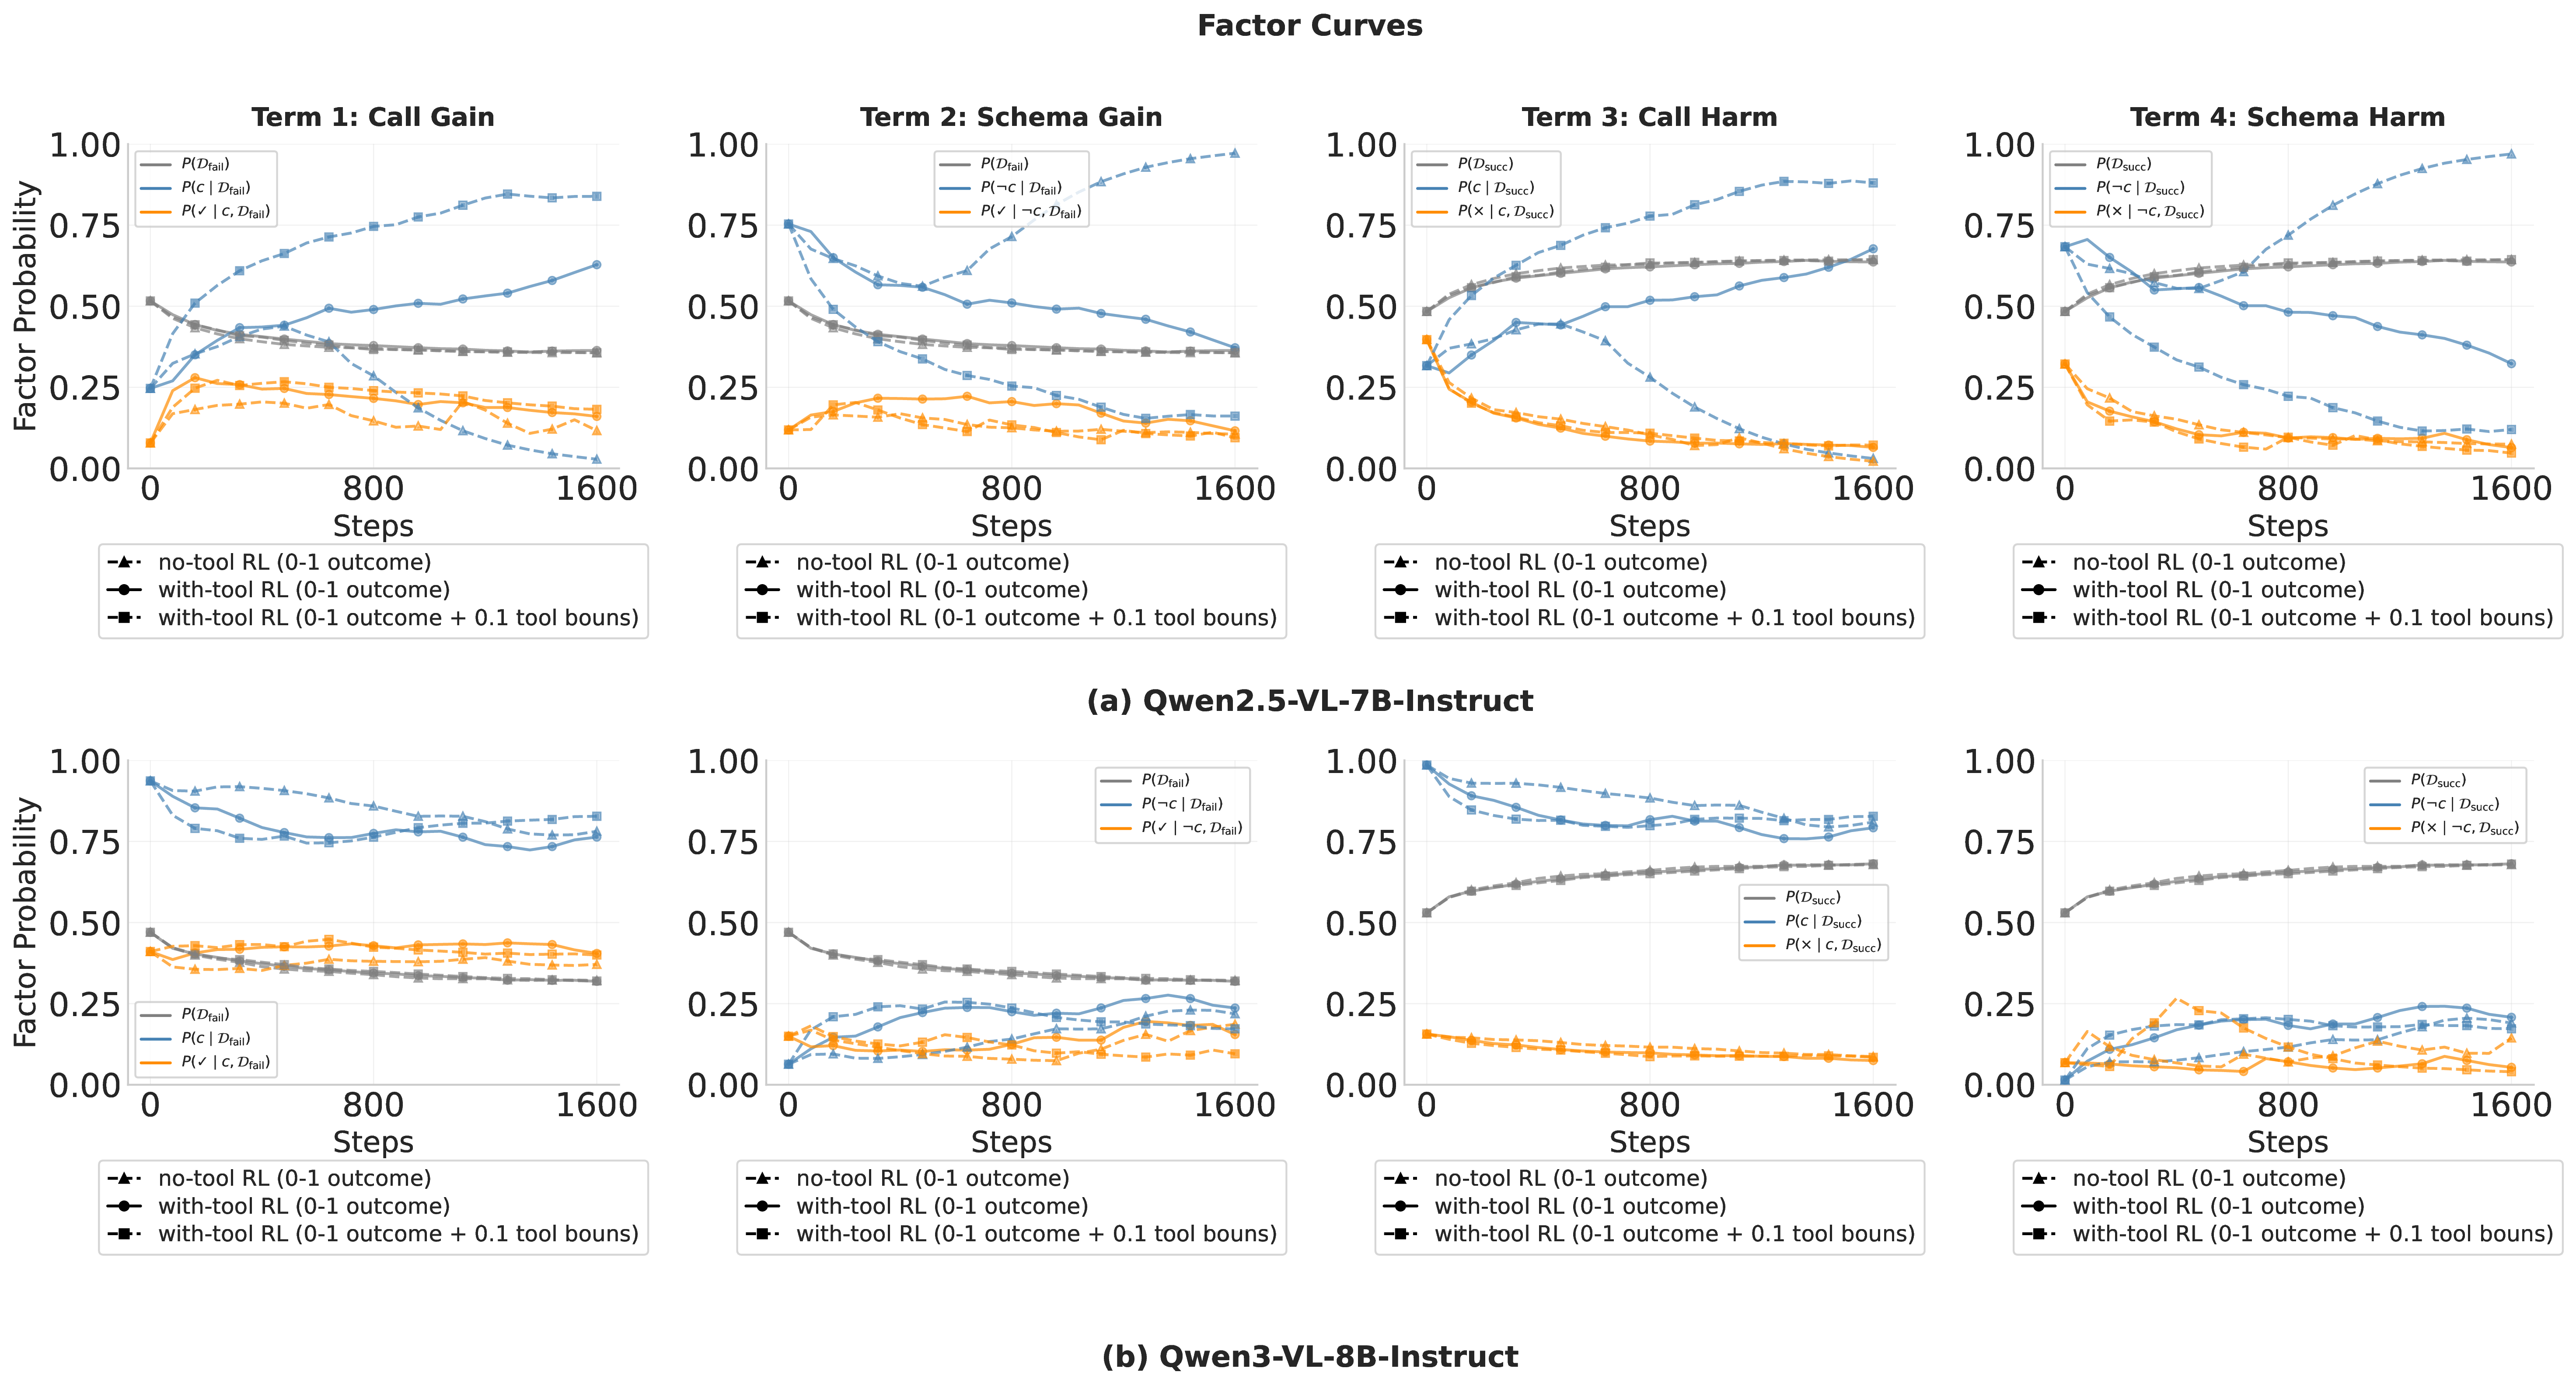
\includegraphics[width=0.98\linewidth]{figures/paper3/baseline_ablation_qwen25vl_qwen3vl_diagnose_term_comparison_factors.png}
\end{frame}

\begin{frame}{\Large Backup: EXP-I Per Bench Qwen2.5VL}
  \centering
  \vspace{0.12cm}
  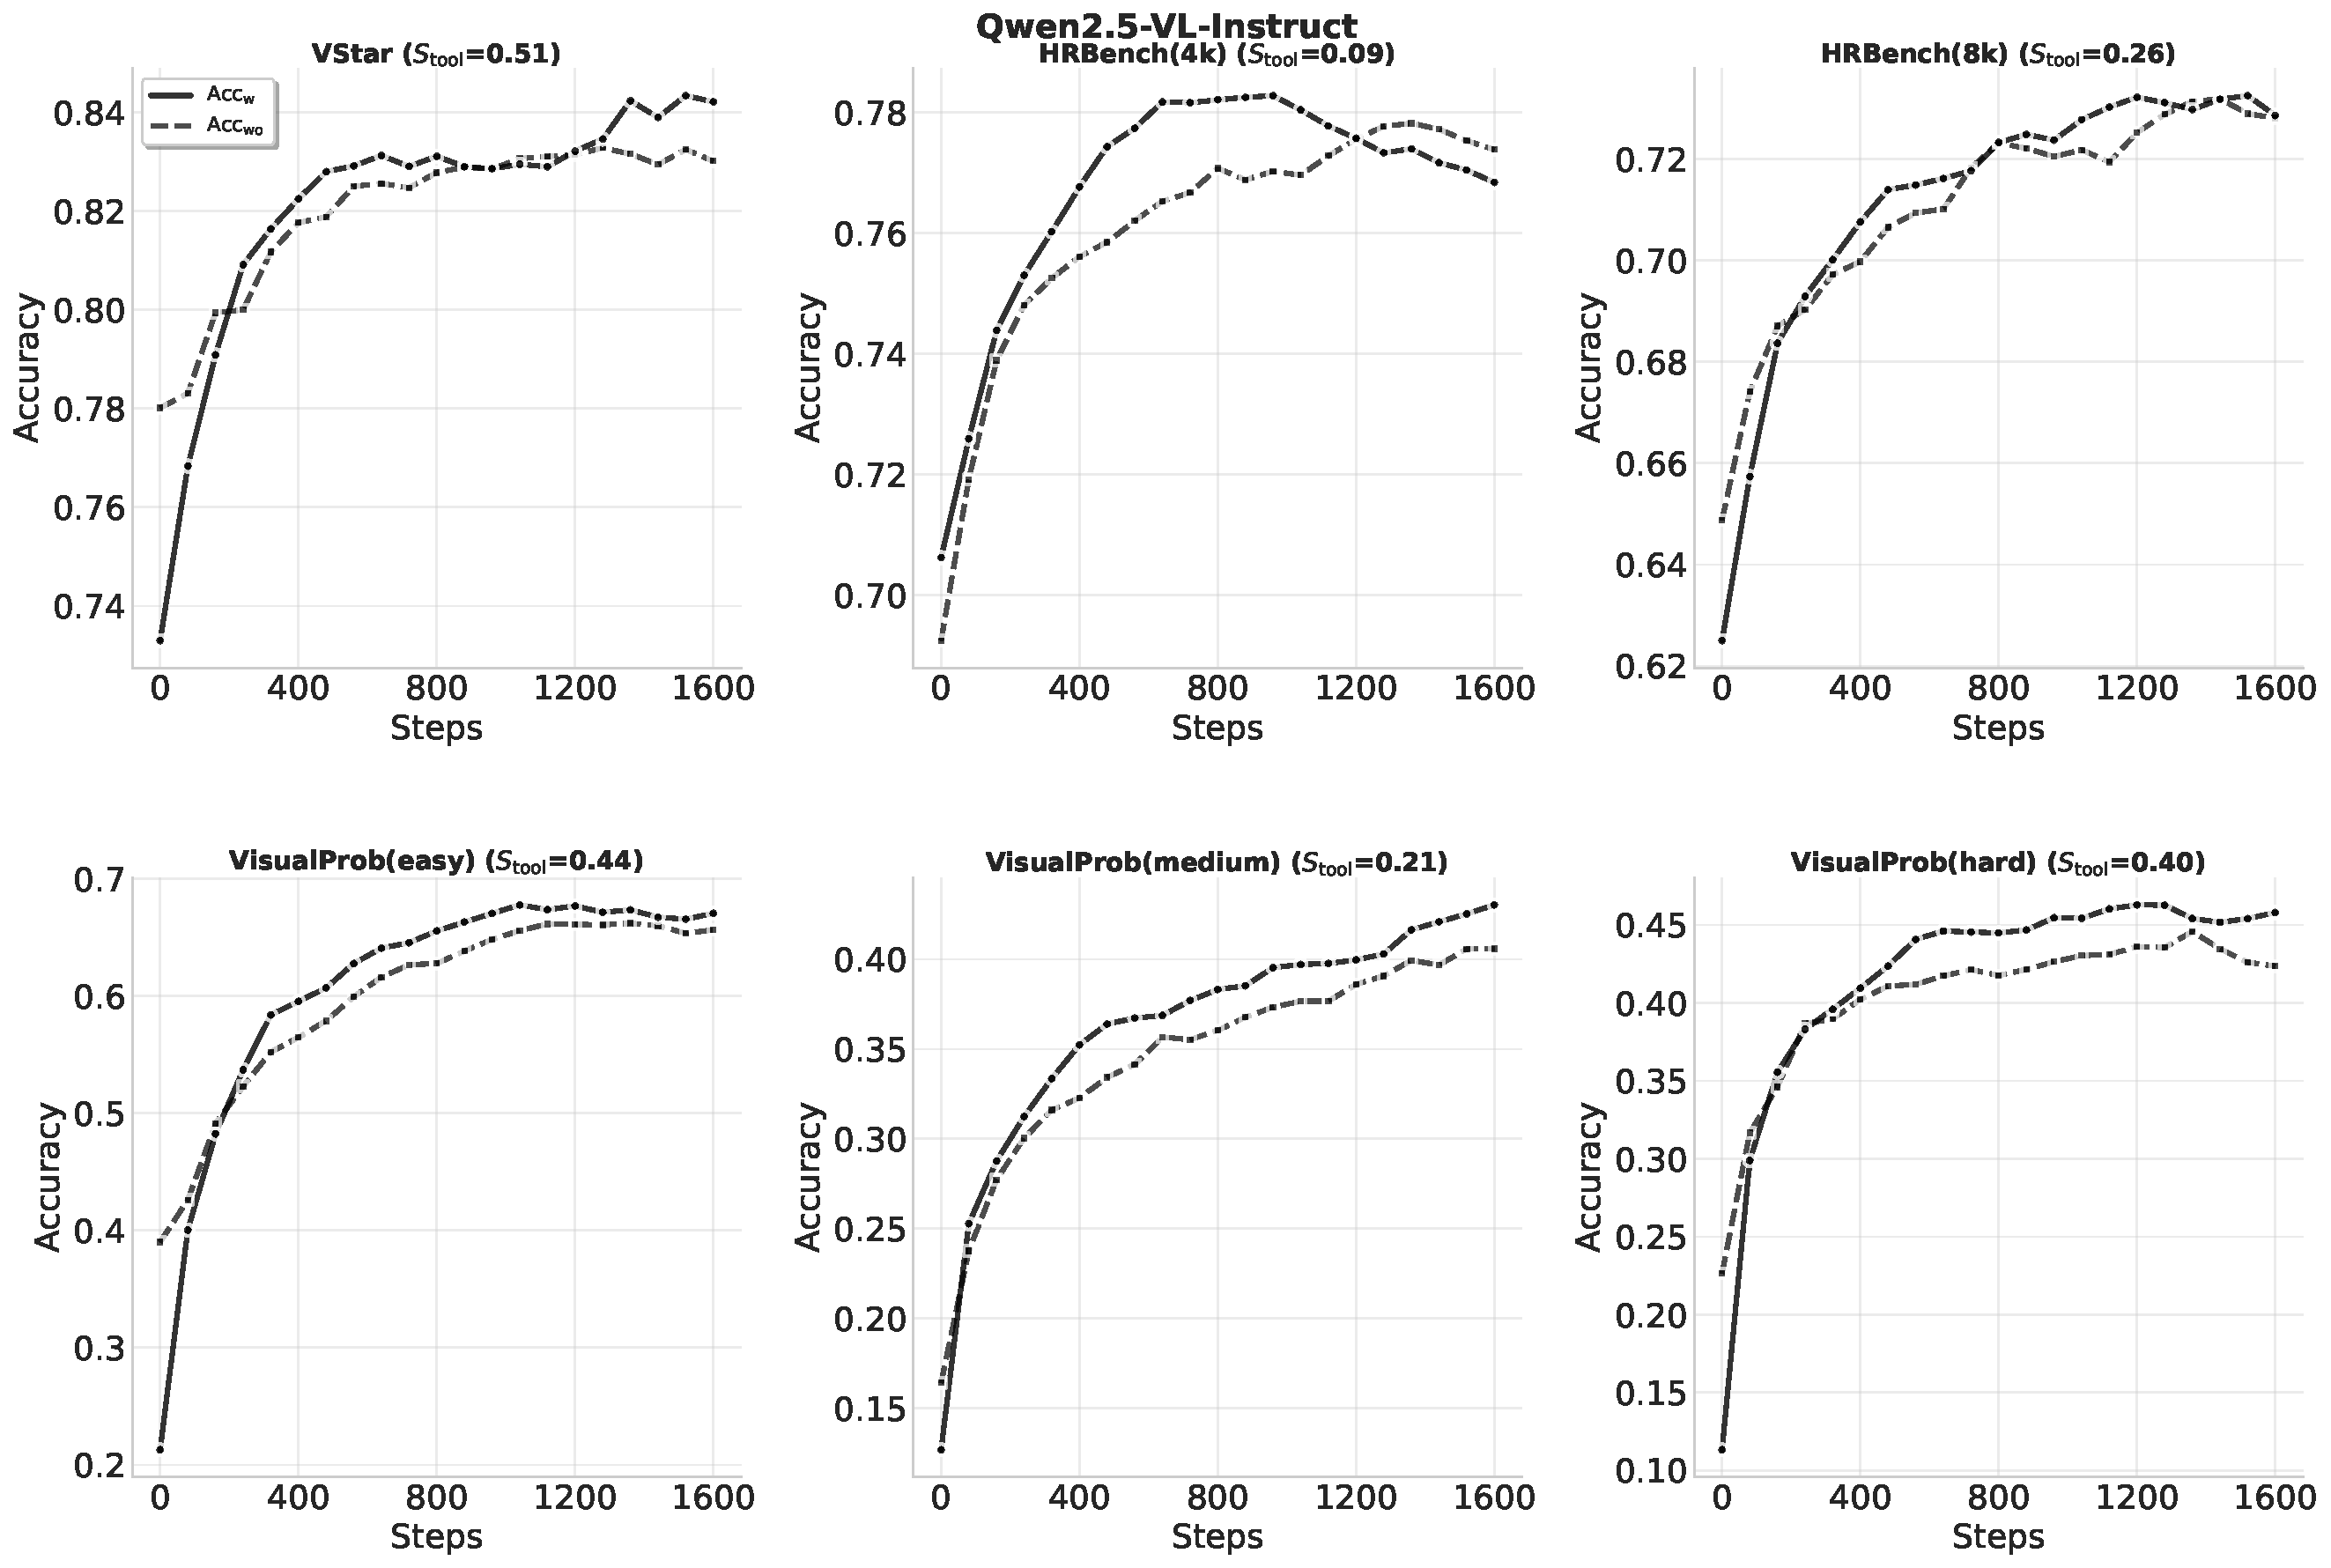
\includegraphics[width=0.80\linewidth]{figures/paper3/exp1_per_benchmark_qwen25vl.pdf}
\end{frame}

\begin{frame}{\Large Backup: EXP-I Per Bench Qwen3VL}
  \centering
  \vspace{0.12cm}
  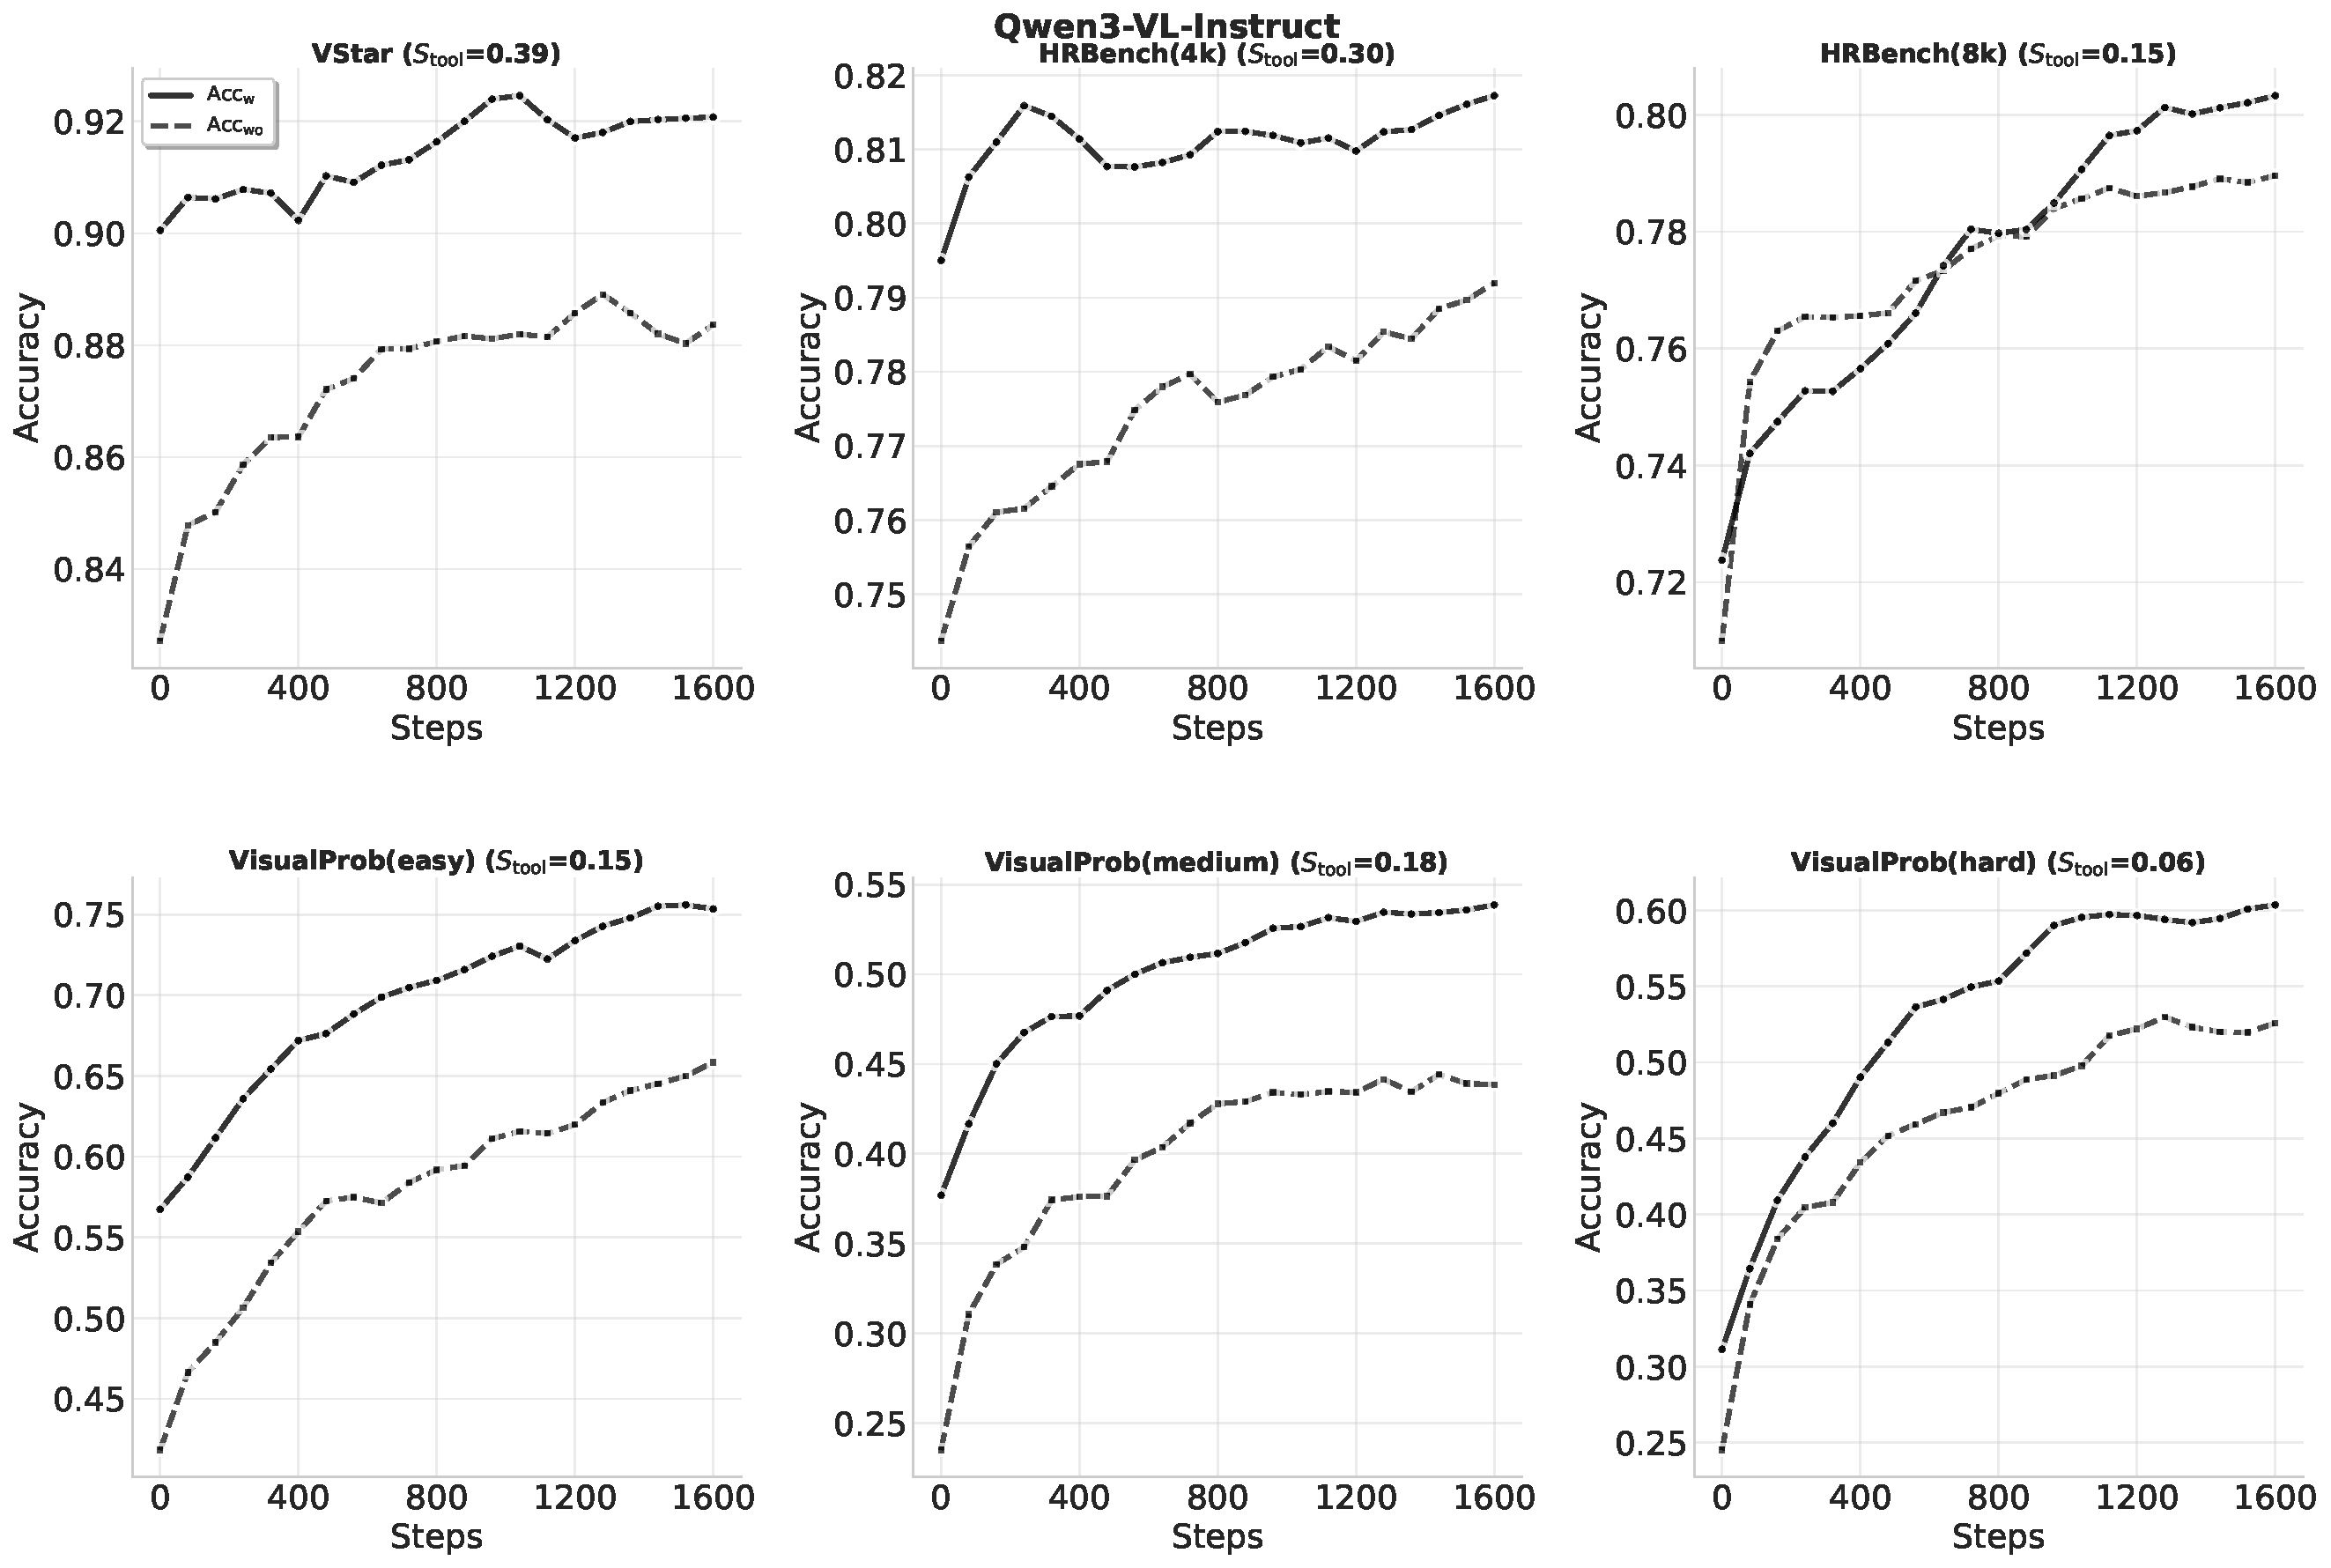
\includegraphics[width=0.80\linewidth]{figures/paper3/exp1_per_benchmark_qwen3vl.pdf}
\end{frame}

\begin{frame}{\Large Backup: EXP-II Per Bench Qwen2.5VL}
  \centering
  \vspace{0.12cm}
  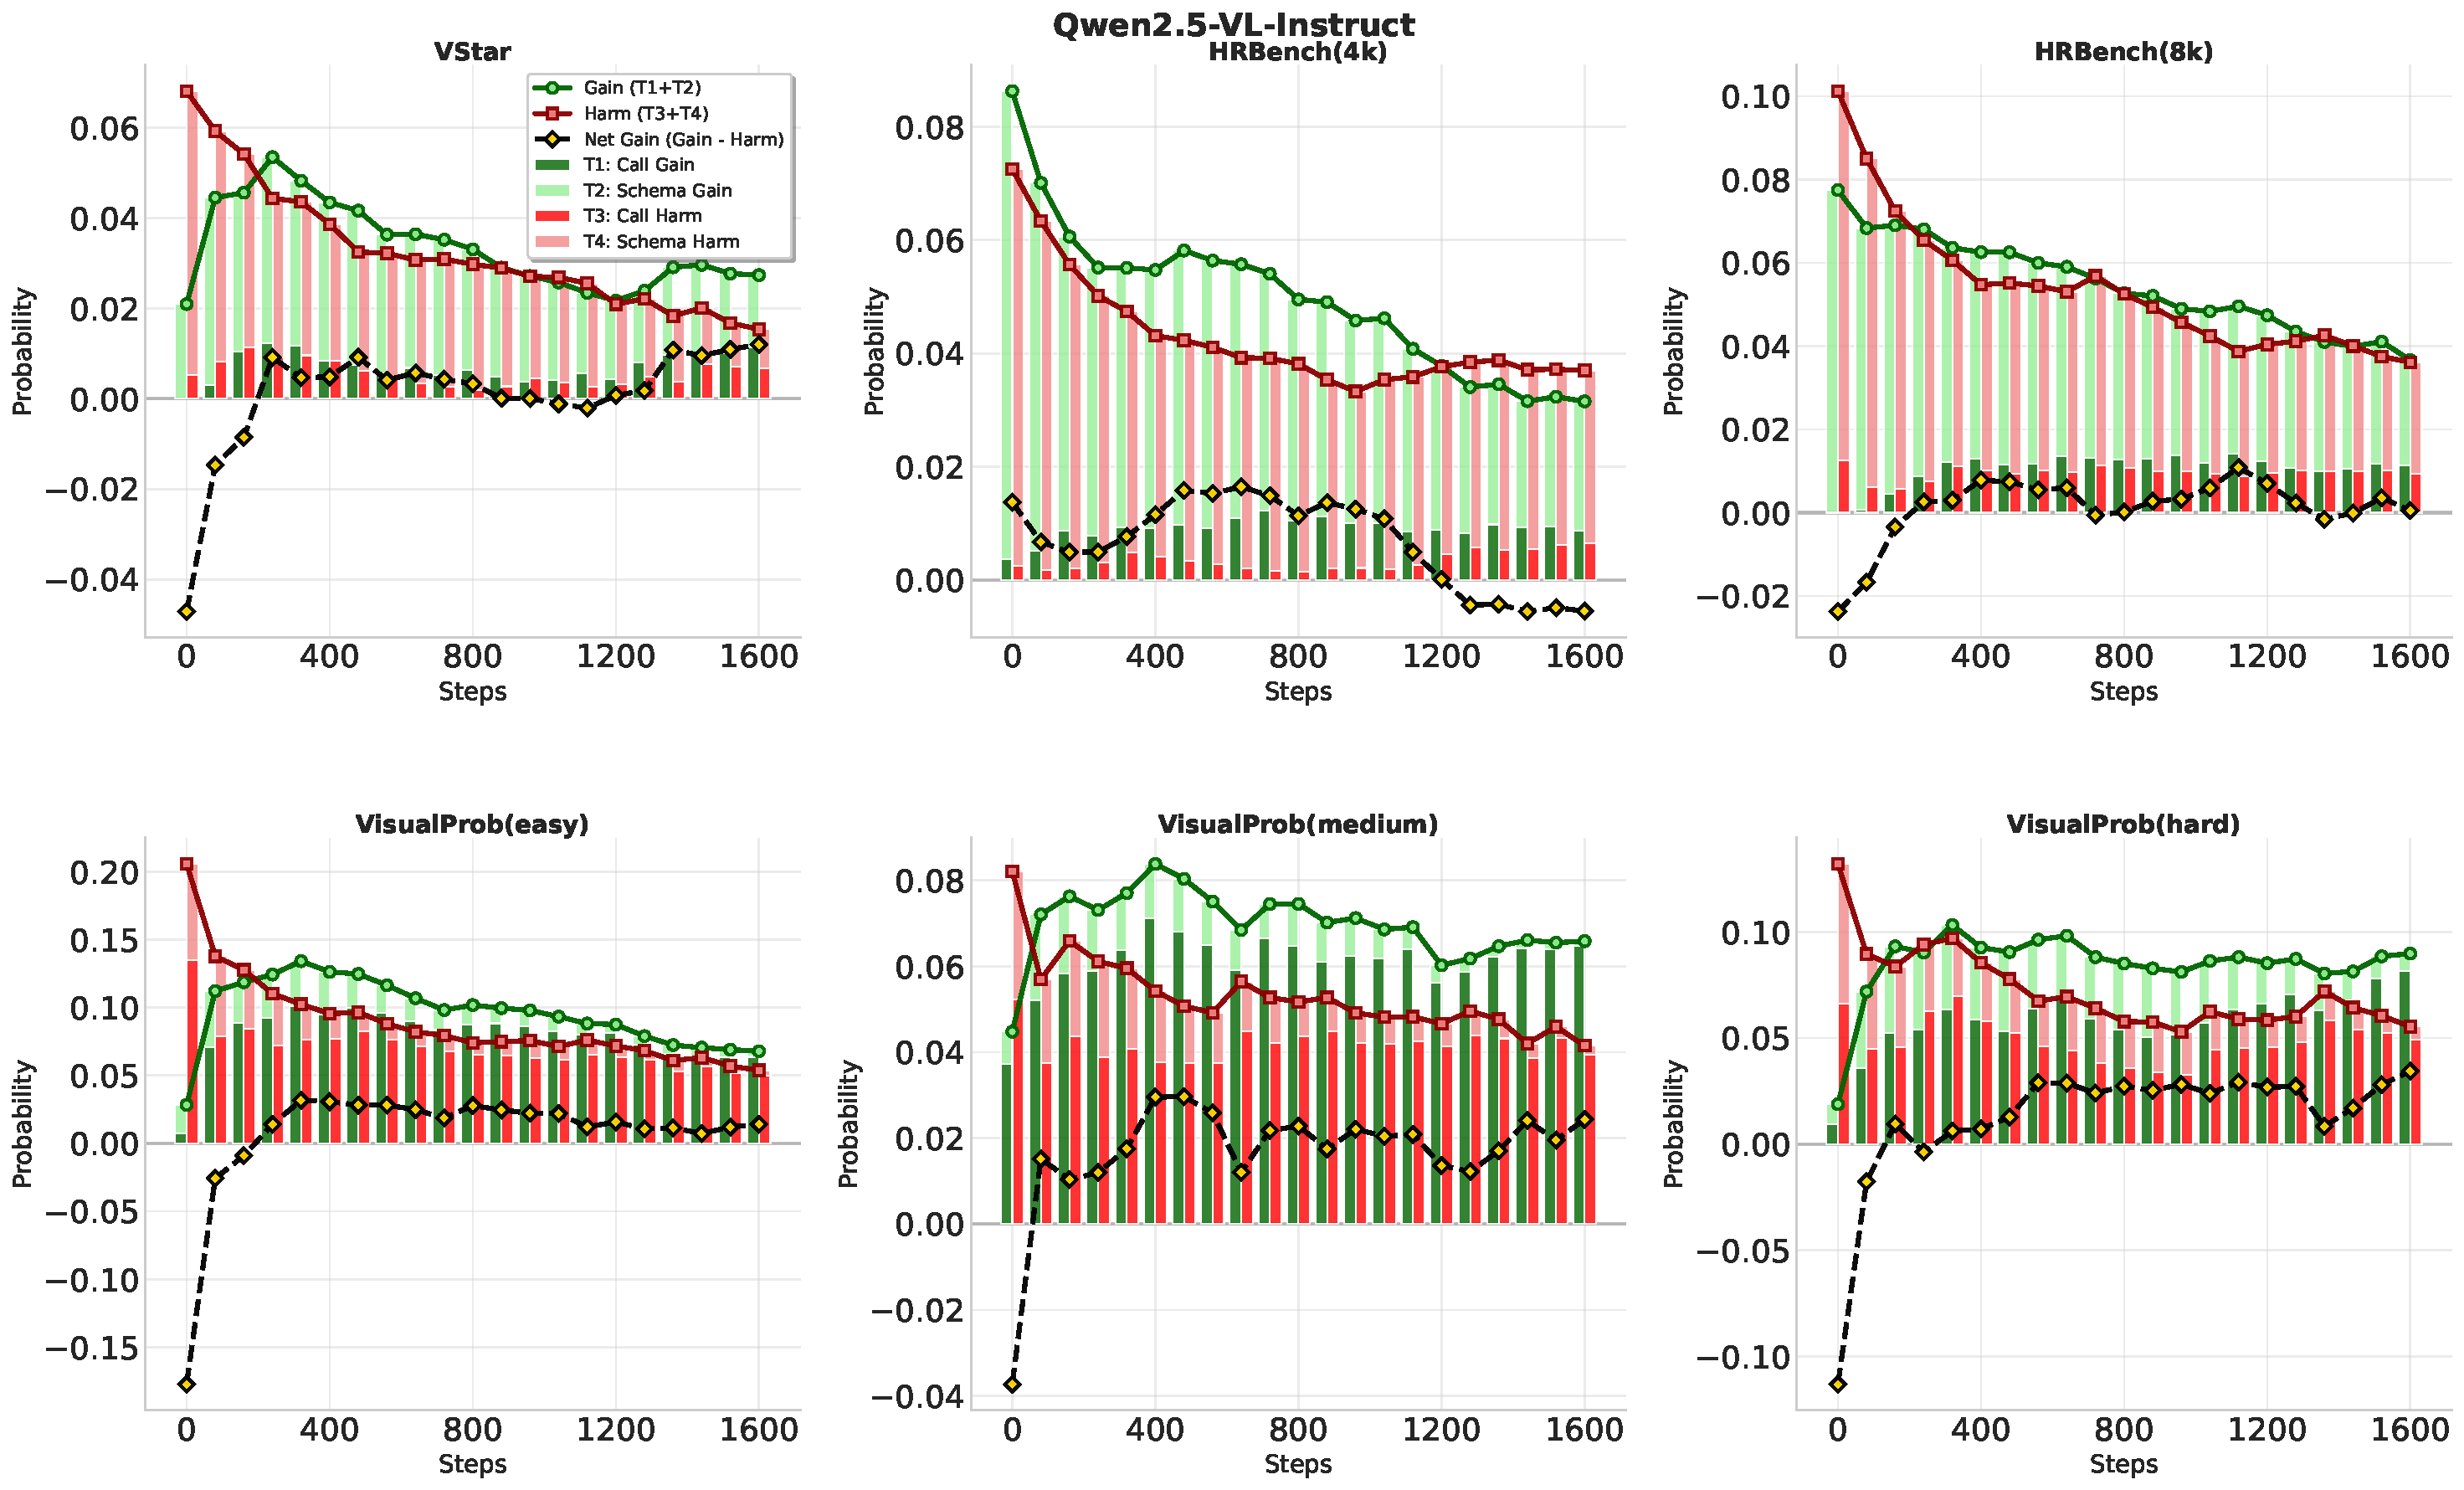
\includegraphics[width=0.80\linewidth]{figures/paper3/exp2_per_benchmark_qwen25vl.pdf}
\end{frame}

\begin{frame}{\Large Backup: EXP-II Per Bench Qwen3VL}
  \centering
  \vspace{0.12cm}
  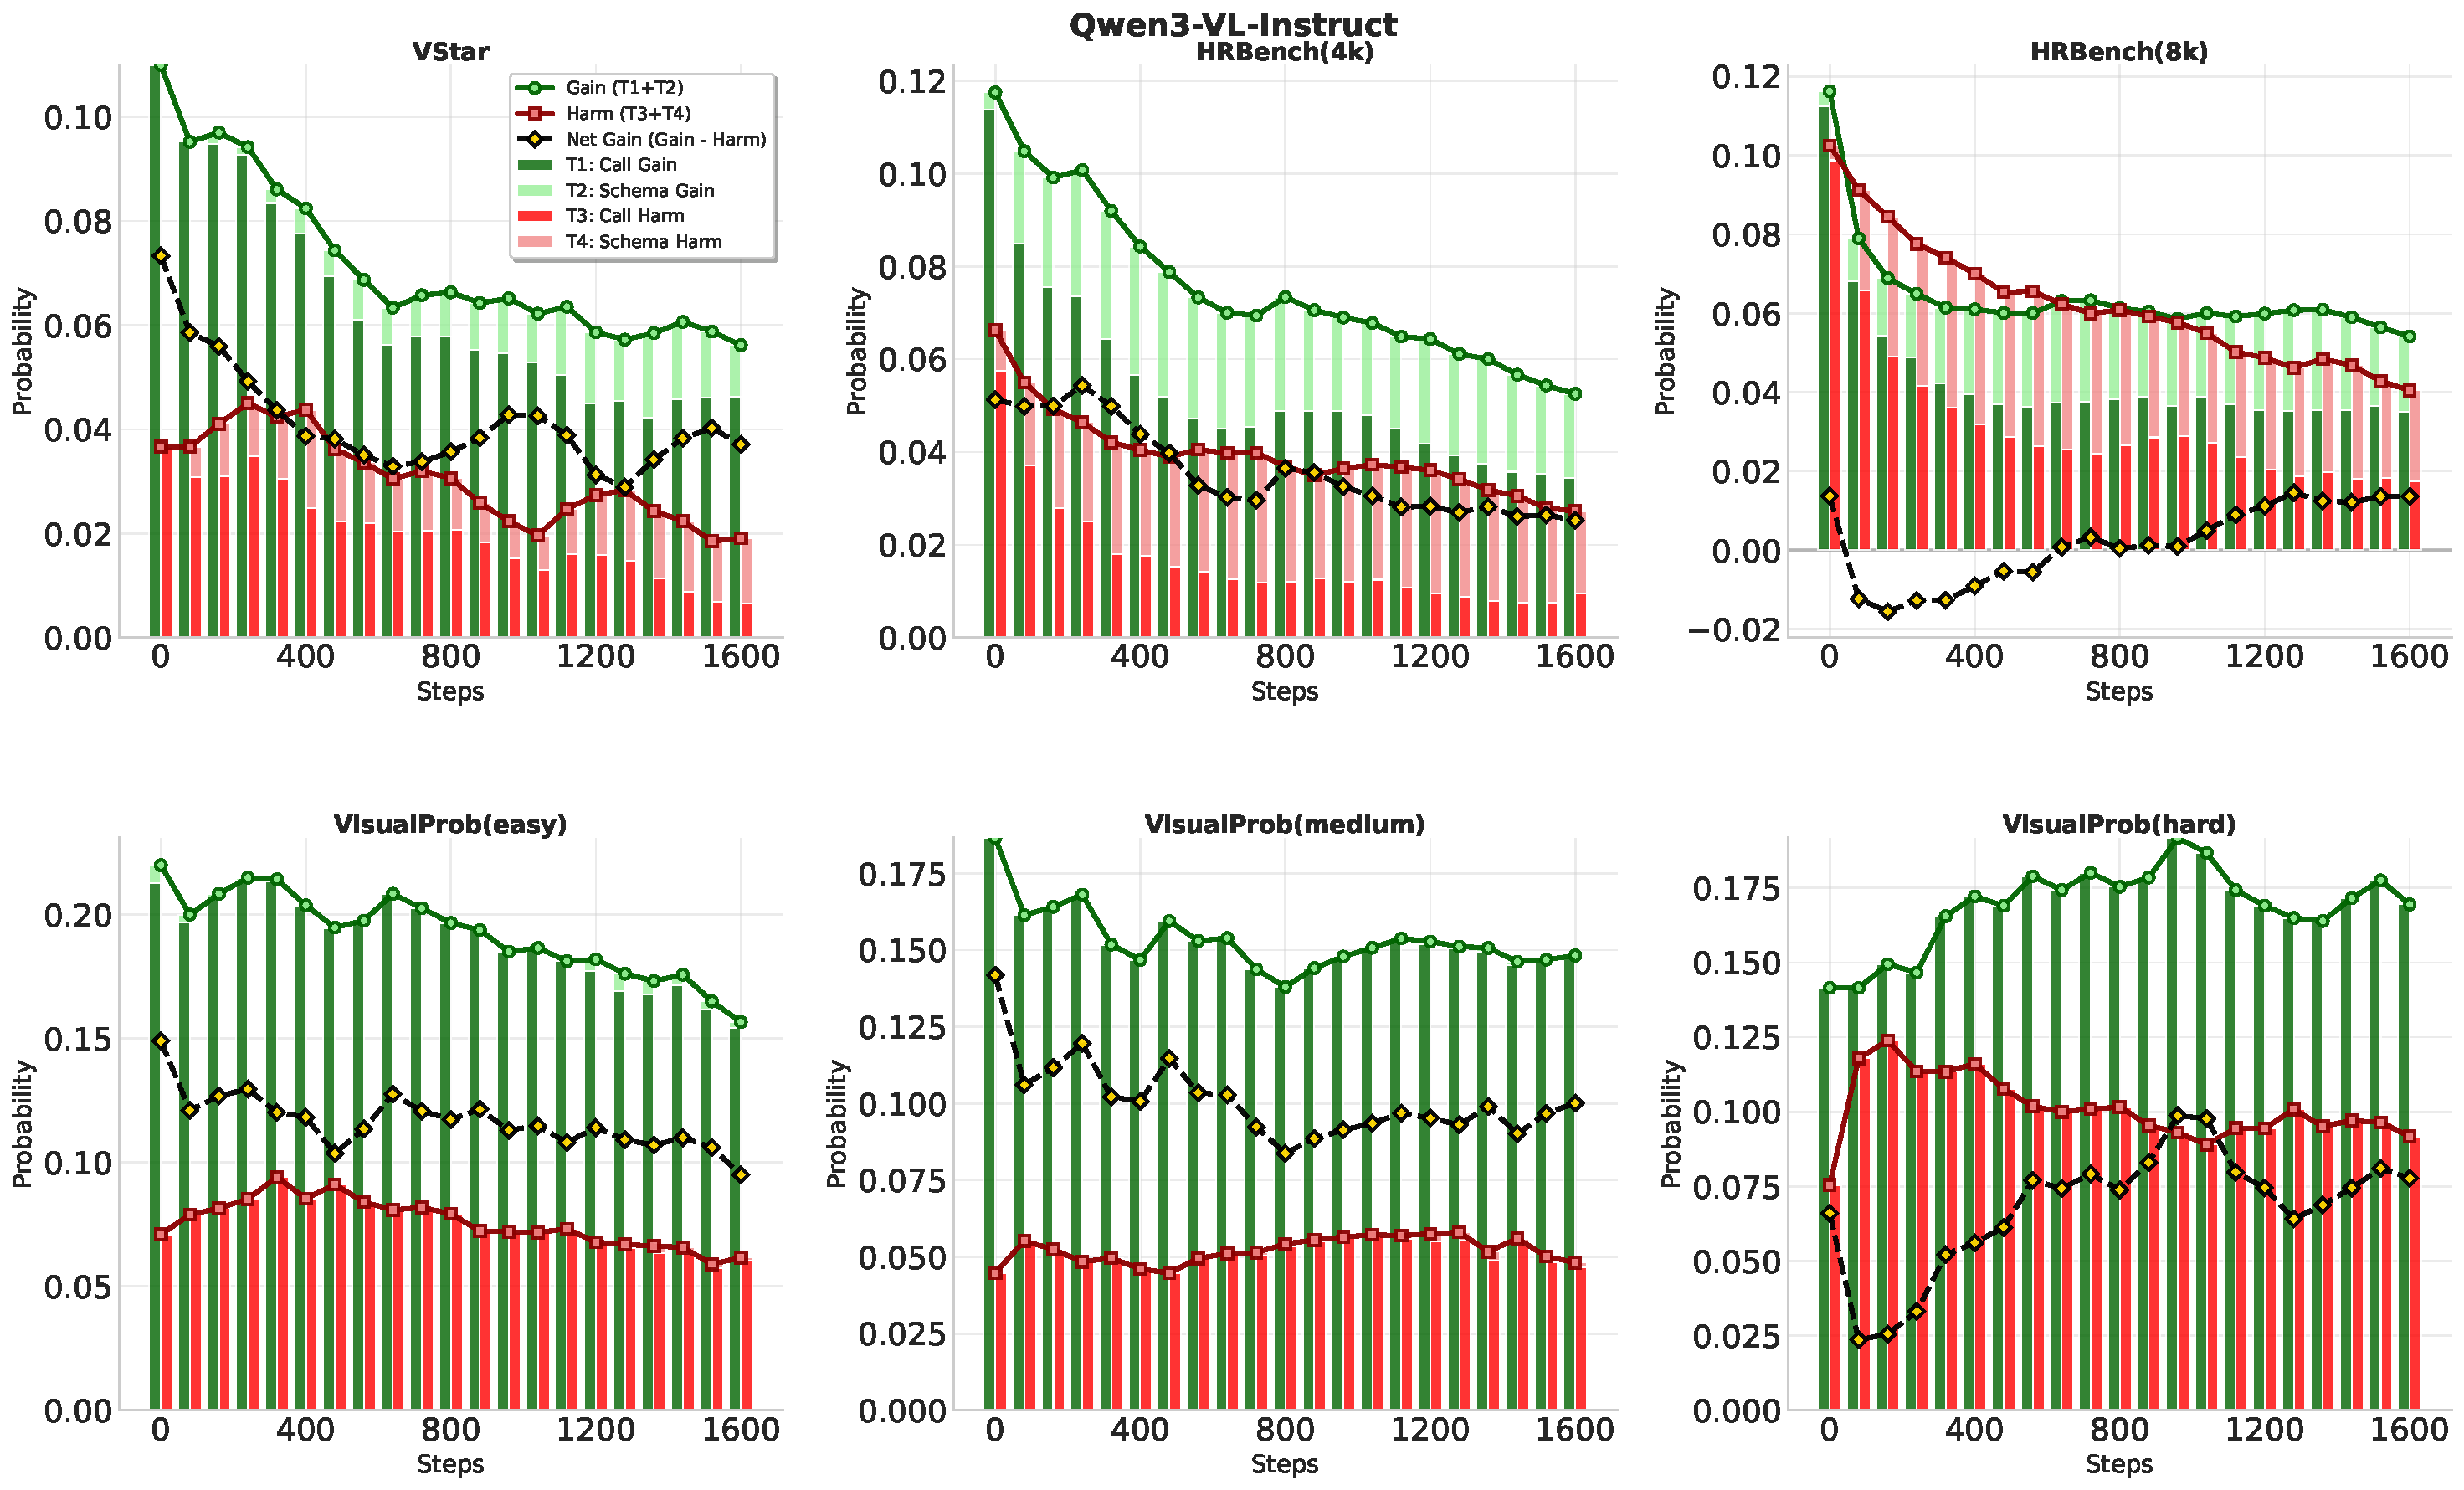
\includegraphics[width=0.80\linewidth]{figures/paper3/exp2_per_benchmark_qwen3vl.pdf}
\end{frame}

\begin{frame}{\Large Backup: EXP-III Per Bench Qwen2.5VL}
  \centering
  \vspace{0.12cm}
  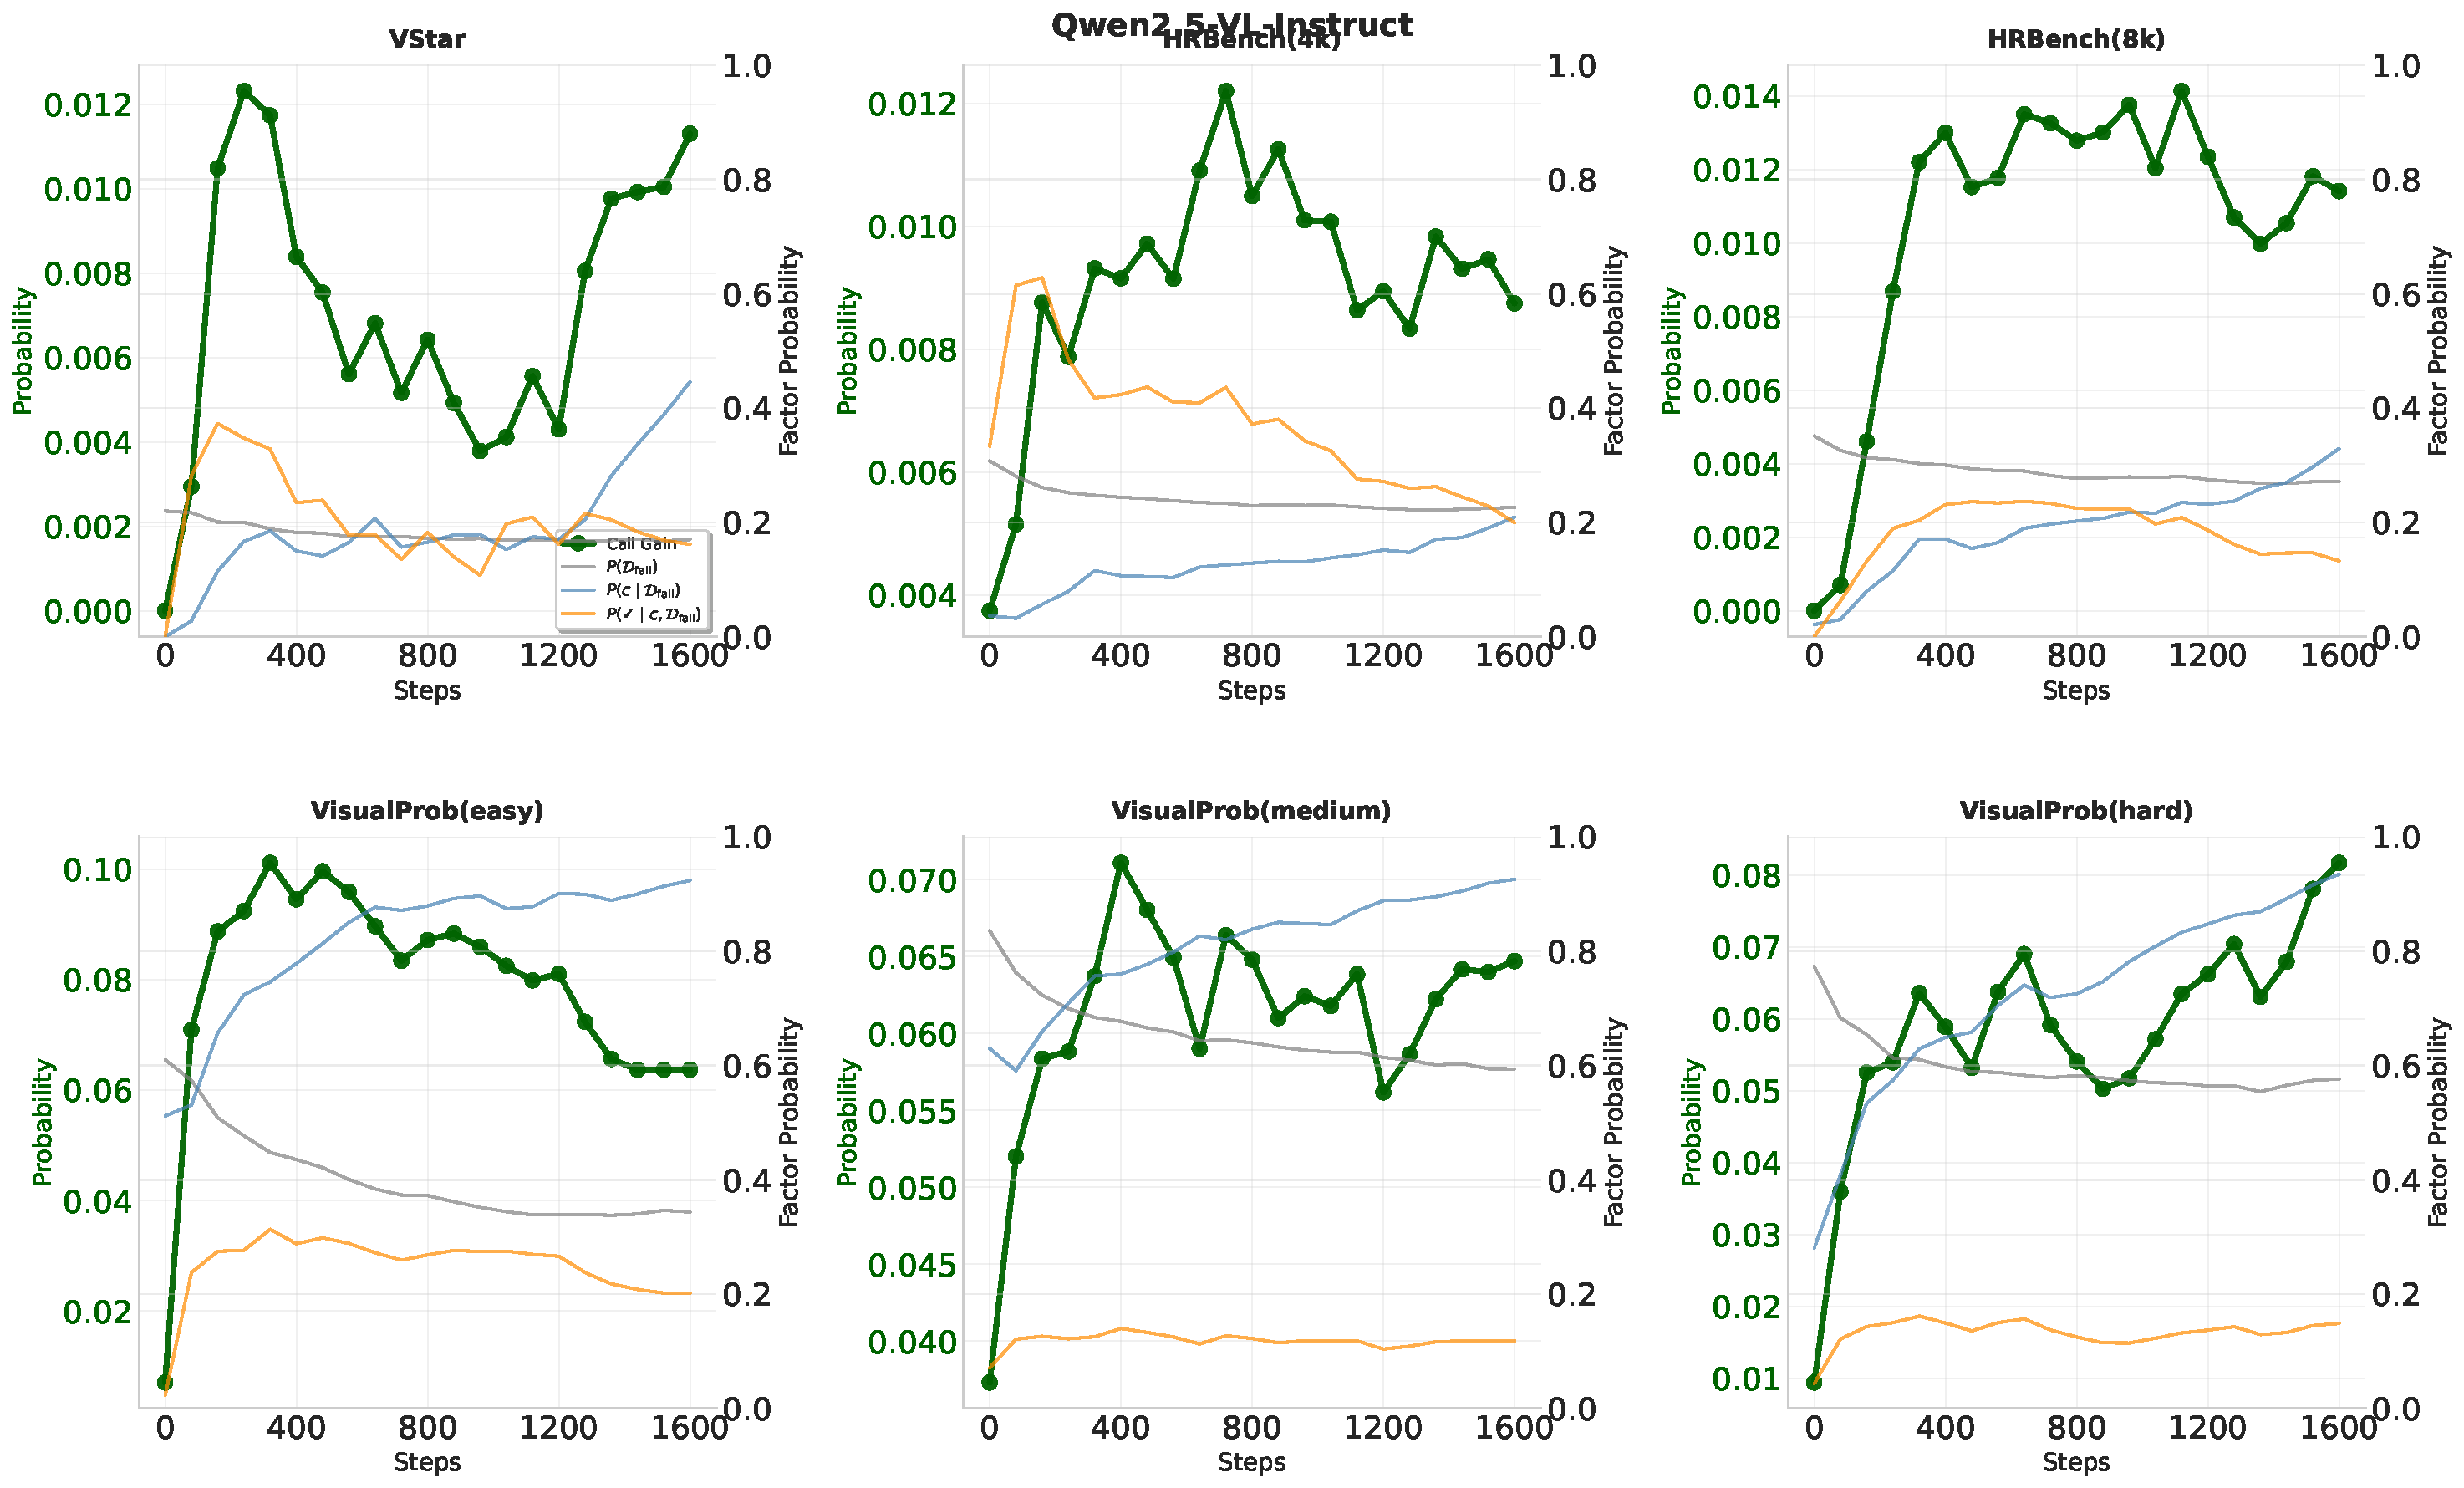
\includegraphics[width=0.80\linewidth]{figures/paper3/exp3_per_benchmark_qwen25vl.pdf}
\end{frame}

\begin{frame}{\Large Backup: EXP-III Per Bench Qwen3VL}
  \centering
  \vspace{0.12cm}
  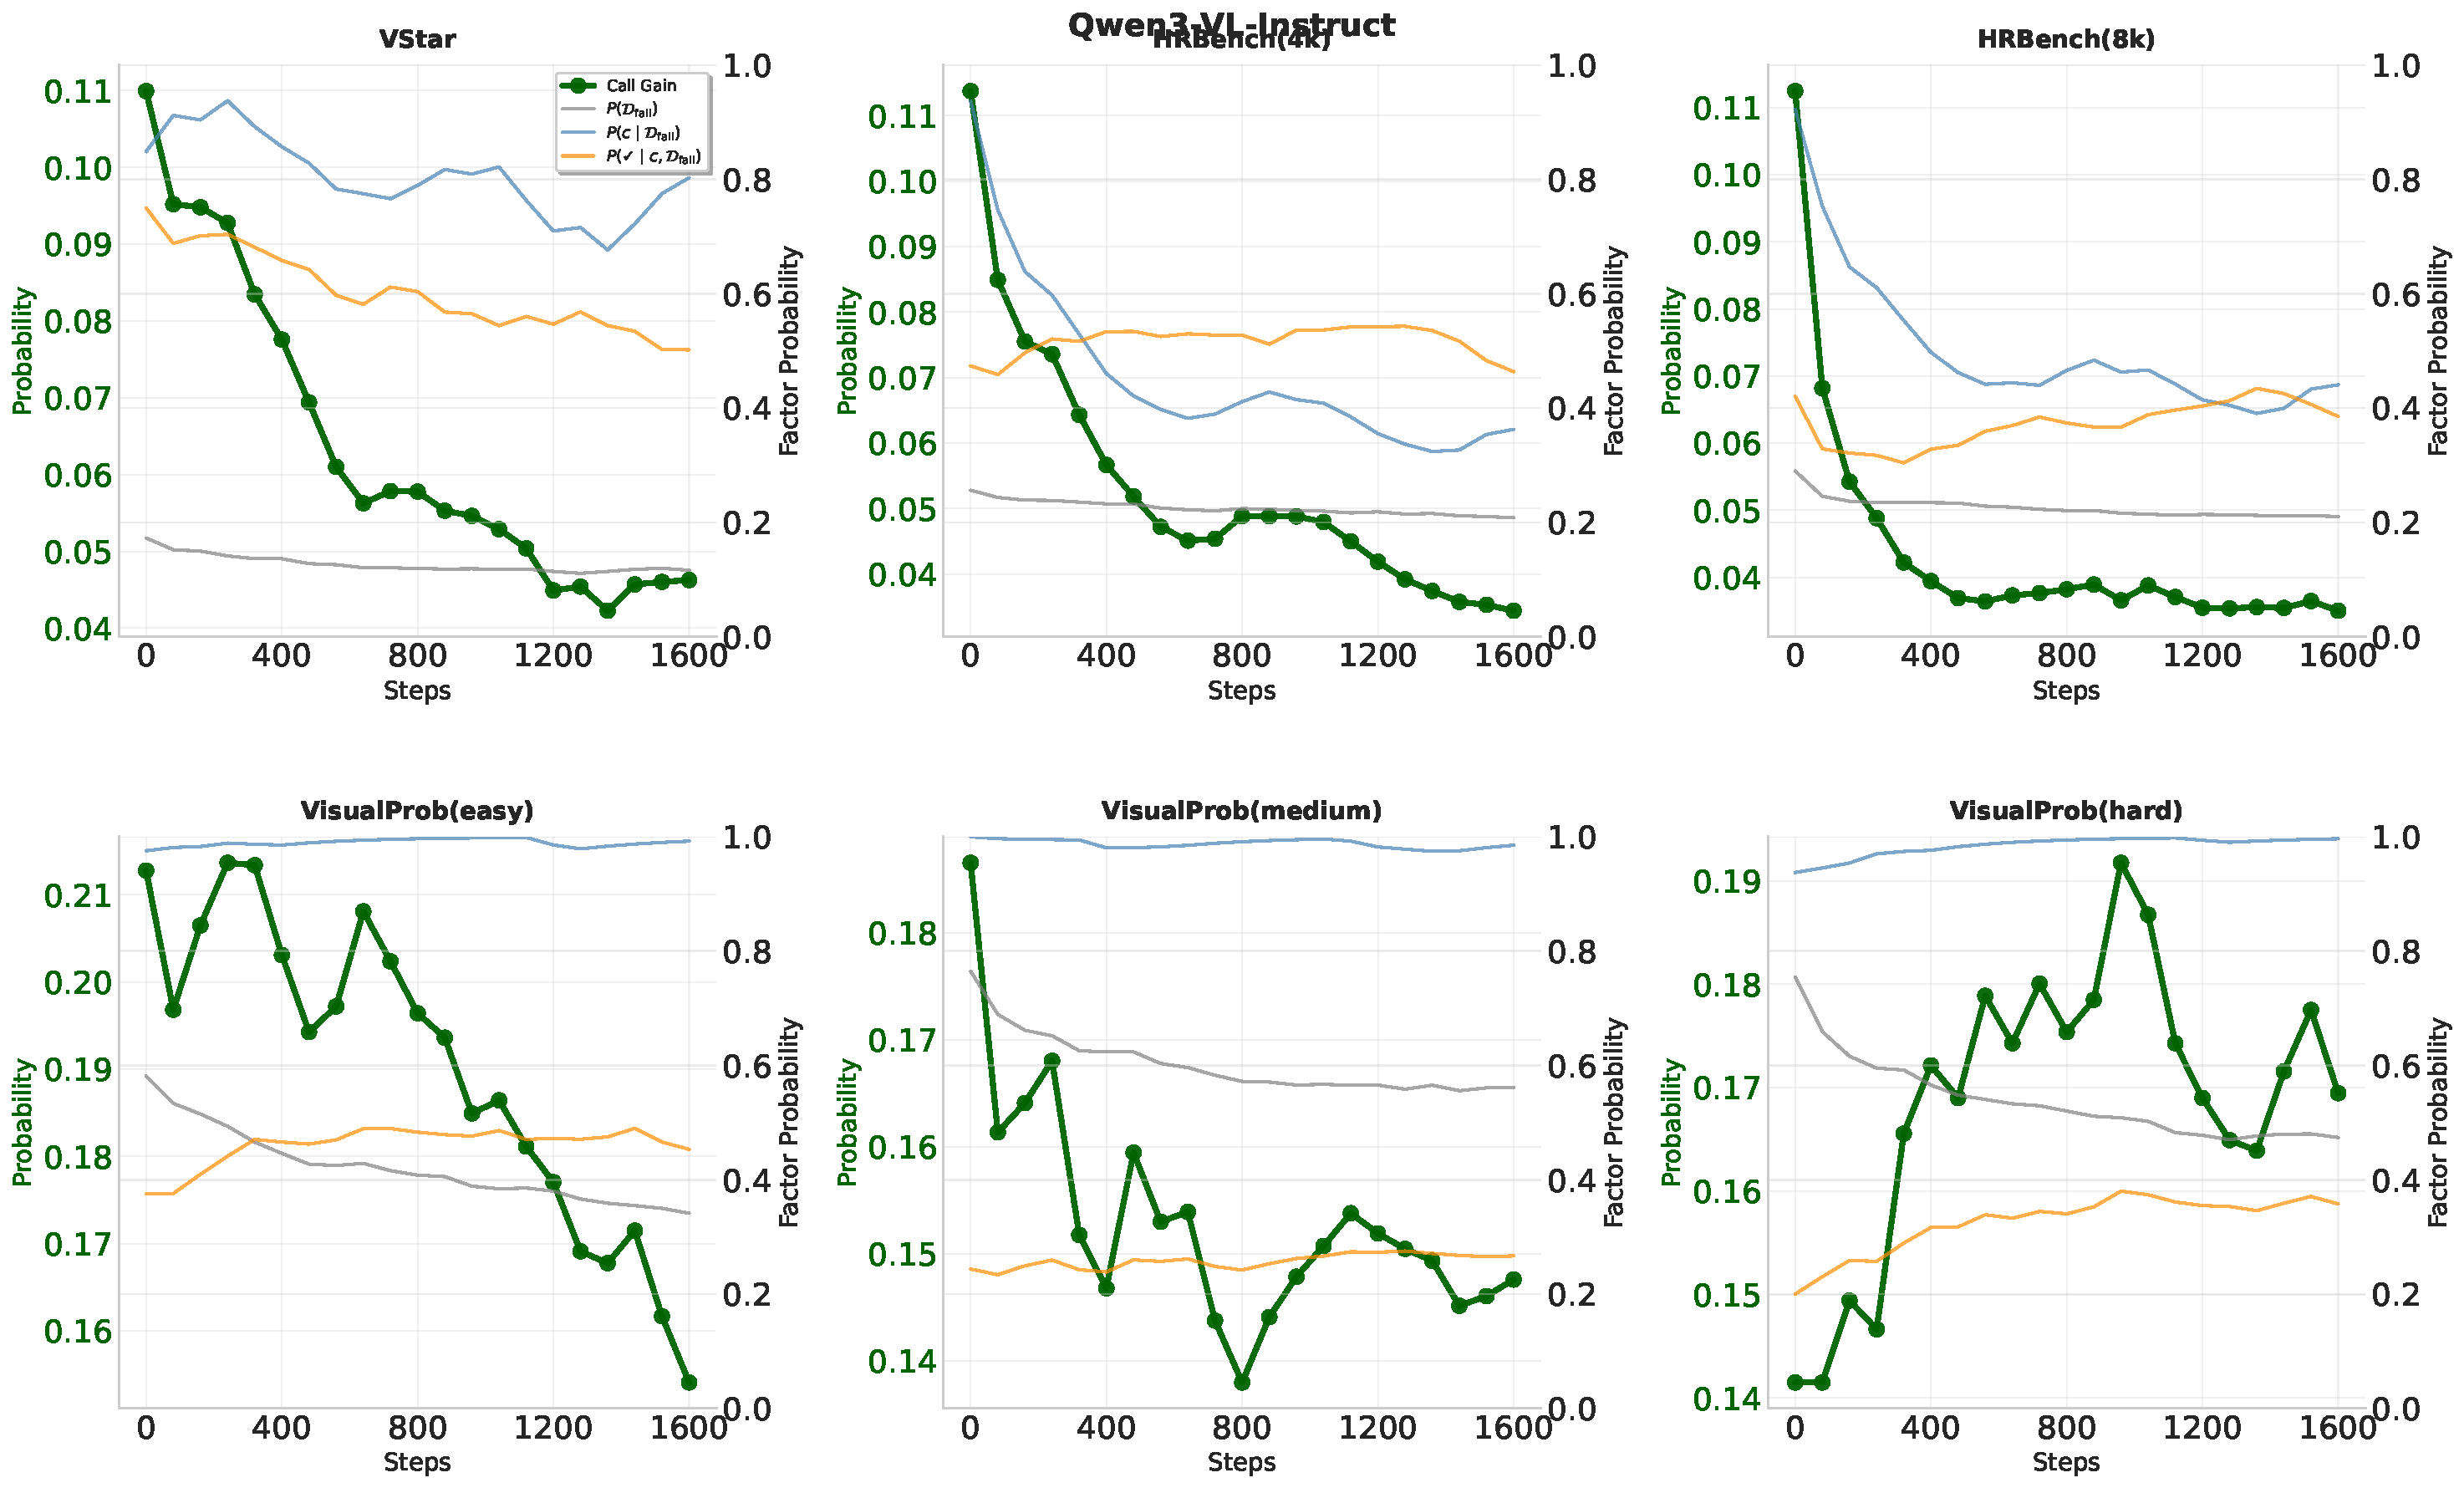
\includegraphics[width=0.80\linewidth]{figures/paper3/exp3_per_benchmark_qwen3vl.pdf}
\end{frame}

\begin{frame}{\Large Backup: Research Lens}
  \centering
  \vspace{-0.08cm}
  \begin{tikzpicture}
    \node[inner sep=0pt] (lens) at (0,0) {
      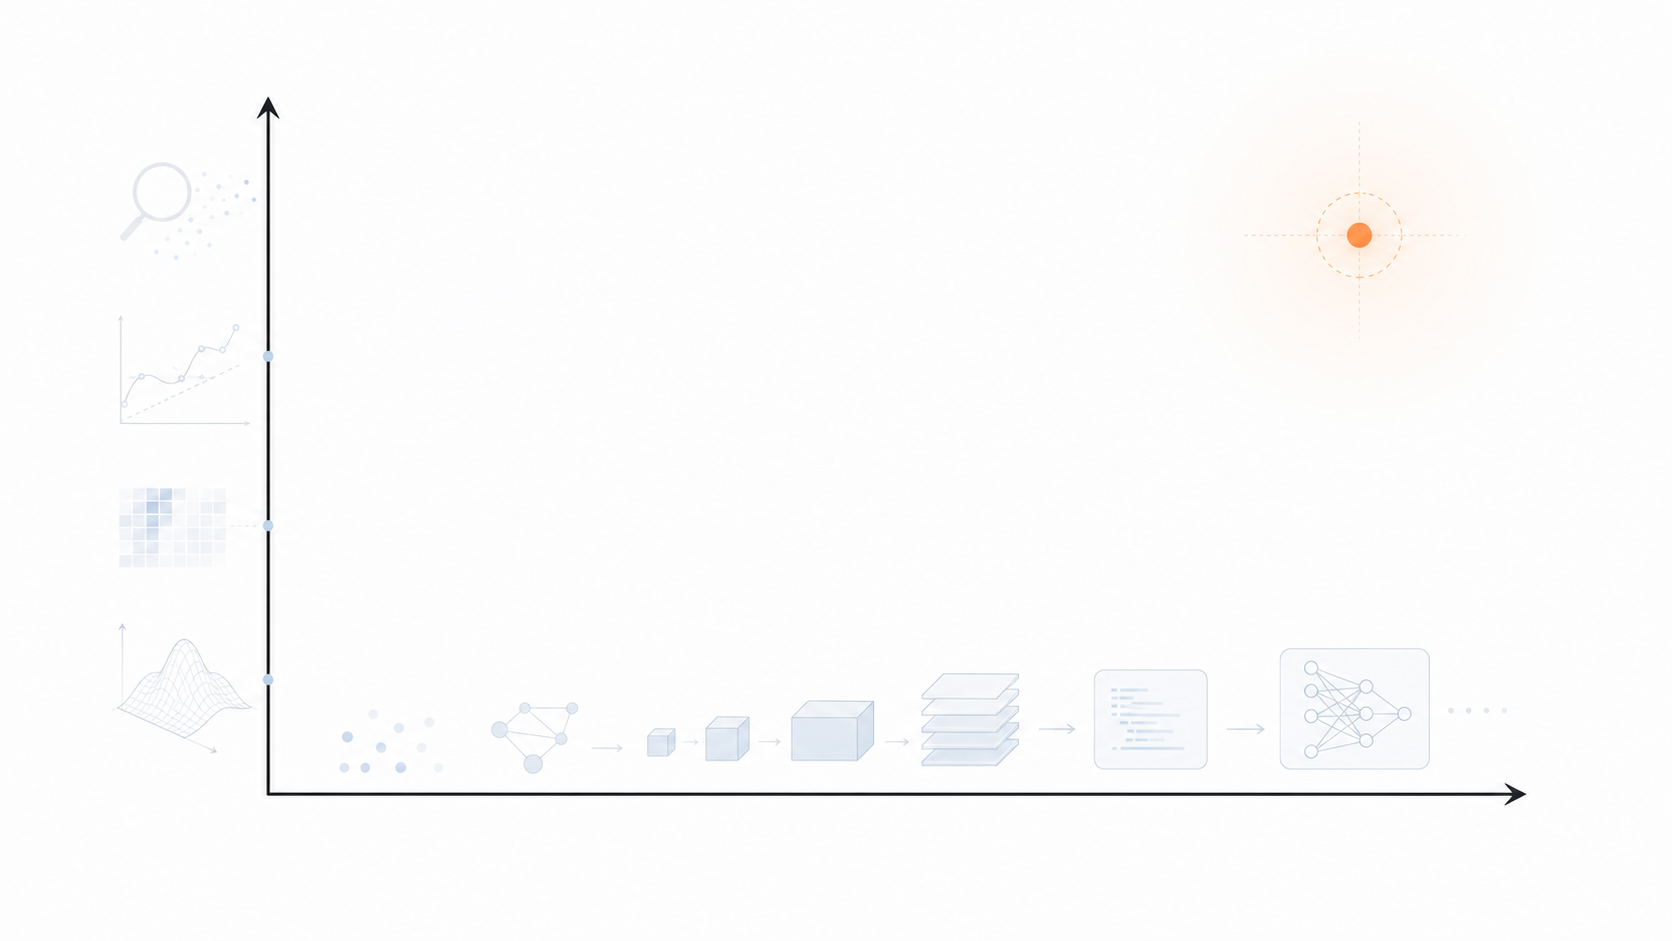
\includegraphics[width=0.98\linewidth]{figures/reasearch_lens.png}
    };

    \node[
      anchor=south,
      font=\small\bfseries
    ] at ([xshift=2.45cm,yshift=0.50cm]lens.south) {Engineering Capability};

    \node[
      rotate=90,
      anchor=south,
      font=\small\bfseries
    ] at ([xshift=-4.00cm,yshift=0.30cm]lens.center) {Scientific Understanding};

    \node[
      anchor=west,
      align=left,
      font=\small,
      text=AgentInk
    ] at ([xshift=1.45cm,yshift=1.05cm]lens.center) {
      \textbf{My Interest}\\[-0.15em]
      explaining emerging\\[-0.15em]
      multimodal-agent capabilities
    };

    \node[
      anchor=west,
      align=left,
      font=\scriptsize\itshape,
      text=AgentInk!70
    ] at ([xshift=-6.40cm,yshift=-3.22cm]lens.center) {
      ``Scientists study the world as it is;\\[-0.10em]
      engineers create the world that never has been.''\\[-0.05em]
      \normalfont\scriptsize --- Theodore von K\'arm\'an
    };
  \end{tikzpicture}
\end{frame}
